%%%%%%%%%%%%%%%%%%%%%%%%%%%%%%%%%%%%%%%%%%%%%%%%%%%%%%%%%%%%
%%% ELIFE ARTICLE TEMPLATE
%%%%%%%%%%%%%%%%%%%%%%%%%%%%%%%%%%%%%%%%%%%%%%%%%%%%%%%%%%%%
%%% PREAMBLE
\documentclass[9pt,lineno]{elife}
% Use the onehalfspacing option for 1.5 line spacing
% Use the doublespacing option for 2.0 line spacing
% Please note that these options may affect formatting.
% Additionally, the use of the \newcommand function should be limited.

\usepackage{lipsum} % Required to insert dummy text
\usepackage[version=4]{mhchem}
\usepackage{siunitx}
\DeclareSIUnit\Molar{M}

%%%%%%%%%%%%%%%%%%%%%%%%%%%%%%%%%%%%%%%%%%%%%%%%%%%%%%%%%%%%
%%% ARTICLE SETUP
%%%%%%%%%%%%%%%%%%%%%%%%%%%%%%%%%%%%%%%%%%%%%%%%%%%%%%%%%%%%
\title{Effects of delayed vaccine development and sequence submission on long-term forecast accuracy of seasonal influenza A/H3N2}
%\title{Faster vaccine development improves the accuracy and precision of long-term forecasts for seasonal influenza A/H3N2}

\author[1*]{John Huddleston}
\author[2]{Trevor Bedford}
\affil[1]{Vaccine and Infectious Disease Division, Fred Hutchinson Cancer Center, Seattle, WA, USA}
\affil[2]{Howard Hughes Medical Institute, Seattle, WA, USA}

\corr{jhuddles@fredhutch.org}{JH}

%%%%%%%%%%%%%%%%%%%%%%%%%%%%%%%%%%%%%%%%%%%%%%%%%%%%%%%%%%%%
%%% ARTICLE START
%%%%%%%%%%%%%%%%%%%%%%%%%%%%%%%%%%%%%%%%%%%%%%%%%%%%%%%%%%%%

\begin{document}

\maketitle

\begin{abstract}
% Words: 316
For the last decade, long-term forecasting models have influenced seasonal influenza vaccine design.
These models attempt to predict which populations circulating at the time of vaccine strain selection will be dominant 12 months later when the vaccine is distributed to the public.
Forecasting models depend on hemagglutinin sequences from the WHO’s Global Influenza Surveillance and Response System to identify currently circulating groups of related strains (clades) and estimate clade fitness for forecasts.
However, the average delay between collection of a hemagglutinin sequence and its submission to the Global Initiative on Sharing All Influenza Data (GISAID) database is 3 months.
Submission delays complicate the already difficult 12-month forecasting problem by reducing our understanding of current clade frequencies at the time of forecasting.
These constraints of a 12-month forecast horizon and 3-month average submission delays create an upper bound on the accuracy of any long-term forecasting model.
The global response to the SARS-CoV-2 pandemic revealed that modern vaccine technology like mRNA vaccines can reduce how far we need to forecast into the future to 6 months or less and that expanded support for sequencing can reduce submission delays to GISAID to 1 month on average.
To determine whether these recent advances could also improve long-term forecasts for seasonal influenza, we quantified the effects of reducing forecast horizons and submission delays on the accuracy of forecasts for A/H3N2 populations.
We found that reducing forecast horizons from 12 months to 6 or 3 months reduced average absolute forecasting errors by 36\% and 56\%, respectively.
Reducing submission delays provided little improvement to forecasting accuracy but decreased the uncertainty in current clade frequencies by 50\%.
These results show the potential to substantially improve the accuracy of existing influenza forecasting models by modernizing influenza vaccine development and increasing global sequencing capacity to match global efforts in response to the SARS-CoV-2 pandemic.
\end{abstract}

\section{Introduction}

Seasonal influenza virus infections cause approximately half a million deaths per year \citep{flufactsheet}.
Vaccination provides the best protection against hospitalization and death, but the rapid evolution of the influenza surface protein hemagglutinin (HA) allows viruses to escape existing immunity and requires regular updates to influenza vaccines \citep{Petrova2018}.
The World Health Organization (WHO) meets twice a year to decide on vaccine updates for the Northern and Southern Hemispheres \citep{Morris2018}.
The dominant influenza vaccine is an inactivated whole virus vaccine grown in chicken eggs \citep{Wong2013} which takes 6 to 8 months to develop and contains a single representative vaccine virus per seasonal influenza subtype including A/H1N1pdm, A/H3N2, and B/Victoria \citep{Morris2018}.
As a result, the WHO must select a single immunologically-representative virus per subtype approximately 12 months before the peak of the next influenza season.
These selections depend on the diversity of currently circulating phylogenetic clades, groups of influenza viruses that all share a recent common ancestor.
The WHO's understanding of that genetic diversity comes from HA sequences collected by the WHO's Global Influenza and Surveillance and Response System (GISRS) \citep{Hay2018} and submitted to the Global Initiative on Sharing All Influenza Data (GISAID) database \citep{gisaid}.
The fastest evolving influenza subtype A/H3N2 accumulates 3--4 HA amino acid substitutions per year \citep{Smith2004} such that the clades circulating 12 months after the vaccine decision can be antigenically distinct from clades that were circulating at the time of the decision.

Given the 12-month delay between the decision to update an influenza vaccine and the peak of the following influenza season, the vaccine composition decision is commonly framed as a long-term forecasting problem \citep{Lassig2017}.
For this reason, the decision process is partially informed by computational models that attempt to predict the genetic composition of seasonal influenza populations 12 months in the future based on current genetic and phenotypic data \citep{Morris2018}.
The earliest of these models predicted future influenza populations from HA sequences alone \citep{Luksza:2014hj,Neher:2014eu,Steinbruck2014}.
Recent models include phenotypic data from serological experiments \citep{Morris2018,Huddleston2020,Meijers2023,Meijers2024}, but these models still heavily rely on HA sequences to determine the diversity of clades circulating at the time of a forecast.
Unfortunately, the average delay between collection of a seasonal influenza A/H3N2 HA sample and submission of its sequence to GISAID had been approximately 3 months in the era prior to the SARS-CoV-2 pandemic (\FIG{model_of_delays_and_horizons}A).
While long-term forecasting models continue to improve technically, the constraints of a 12-month forecast horizon and the availability of enough recent, representative HA sequences in GISAID impose an upper bound on the accuracy of long-term forecasts.

The global response to the SARS-CoV-2 pandemic in 2020 showed the speed with which we can develop new vaccines and capture real-time viral genetic diversity.
Decades of research on mRNA vaccines enabled the development of multiple effective vaccines a year after the emergence of SARS-CoV-2 \citep{Mulligan2020,Baden2021}.
This mRNA-based vaccine platform also enabled the approval of booster vaccines targeting Omicron only 3 months after the recommendation of an Omicron-based vaccine candidate \citep{Grant2023}.
% Additional citation: https://www.who.int/news/item/17-06-2022-interim-statement-on--the-composition-of-current-COVID-19-vaccines
% recommendation on June 17, 2022 -> boosters available by ? or season start on ?
In parallel to vaccine development, expanded funding and capacity building for viral genome sequencing enabled unprecedented dense sampling of a pathogen's genetic diversity over a short period of time \citep{Chen2022}.
By 2021, the average time between collection of a SARS-CoV-2 sample and submission of the sample's genome sequence to GISAID had decreased to approximately 1 month \citep{Brito2022}.
This reduction in submission delays reflects both increased emergency funding and the sustained efforts by more public health organizations to adopt best practices for genomic epidemiology \citep{Kalia2021,Black2020}.
Assessments of SARS-CoV-2 short-term forecasts have shown how such reductions in forecast horizon and submission delays can improve the accuracy of short-term forecasts and real-time estimates of clade frequencies \citep{Abousamra2023}.

These technological and societal changes in response to SARS-CoV-2 suggest that we could realistically expect the same outcomes for seasonal influenza.
Work on mRNA vaccines for influenza viruses dates back over a decade \citep{Petsch2012,Brazzoli2016,Pardi2018,Feldman2019}.
A switch from the current egg-based inactivated virus vaccines to mRNA vaccines could reduce the time between vaccine design decisions and the peak influenza season from 12 months to 6 months.
Similarly, the expanded global capacity for sequencing SARS-CoV-2 genomes could reasonably extend to broader and more rapid genomic surveillance for seasonal influenza, reducing submission delays from 3 months to 1 month on average.
Even in the years immediately after the onset of the SARS-CoV-2 pandemic, we have observed a trend toward a reduced average submission delay of 2.5 months that we would expect from increased global capacity for genome sequencing (\FIGSUPP[model_of_delays_and_horizons]{distribution_of_delays_by_pandemic_era}).

In this work, we tested the effects of similar reductions in forecast horizons and submission delays on the accuracy of long-term forecasts for seasonal influenza.
Building on our previously published forecasting framework \citep{Huddleston2020}, we performed a retrospective analysis of HA sequences from simulated and natural A/H3N2 populations.
For each population type, we produced forecasts from 12, 9, 6, and 3 months prior to a given influenza season (\FIG{model_of_delays_and_horizons}A).
We made each forecast under three different submission delay scenarios including a realistic delay (3 months on average), an ideal delay (1 month on average), and no delay (\FIG{model_of_delays_and_horizons}B).
First, we measured the accuracy and precision of forecasts under these different scenarios by calculating the genetic distance between predicted and observed future populations using the same earth mover's distance metric that we originally used to train our forecasting models \citep{Rubner1998}.
Next, we calculated the effect of forecast horizon and submission delays on clade frequencies which are the values we use to communicate predictions to WHO decision-makers \citep{Huddleston2024}.
We quantified the effect of reduced submission delays on initial clade frequencies, and we calculated forecast accuracy as the difference between predicted and observed clade frequencies of future populations.
Finally, we calculated the relative improvement in forecast accuracy produced by different realistic interventions including reduced vaccine development time, reduced submission delays, and the combination of both.
In this way, we show the potential to improve the accuracy of existing long-term forecasting models and, thereby, the quality of vaccine design decisions by simplifying the forecasting problem through realistic societal changes.

% Additional interventions to consider from the forecasting model perspective:
% 1. Forecast from the same start point to the beginning of the flu season (e.g., 9 months instead of 12 months into the future)
% 2. Forecast from N weeks earlier than the current date to have more reliable estimates of population composition

\begin{figure}[htb!]
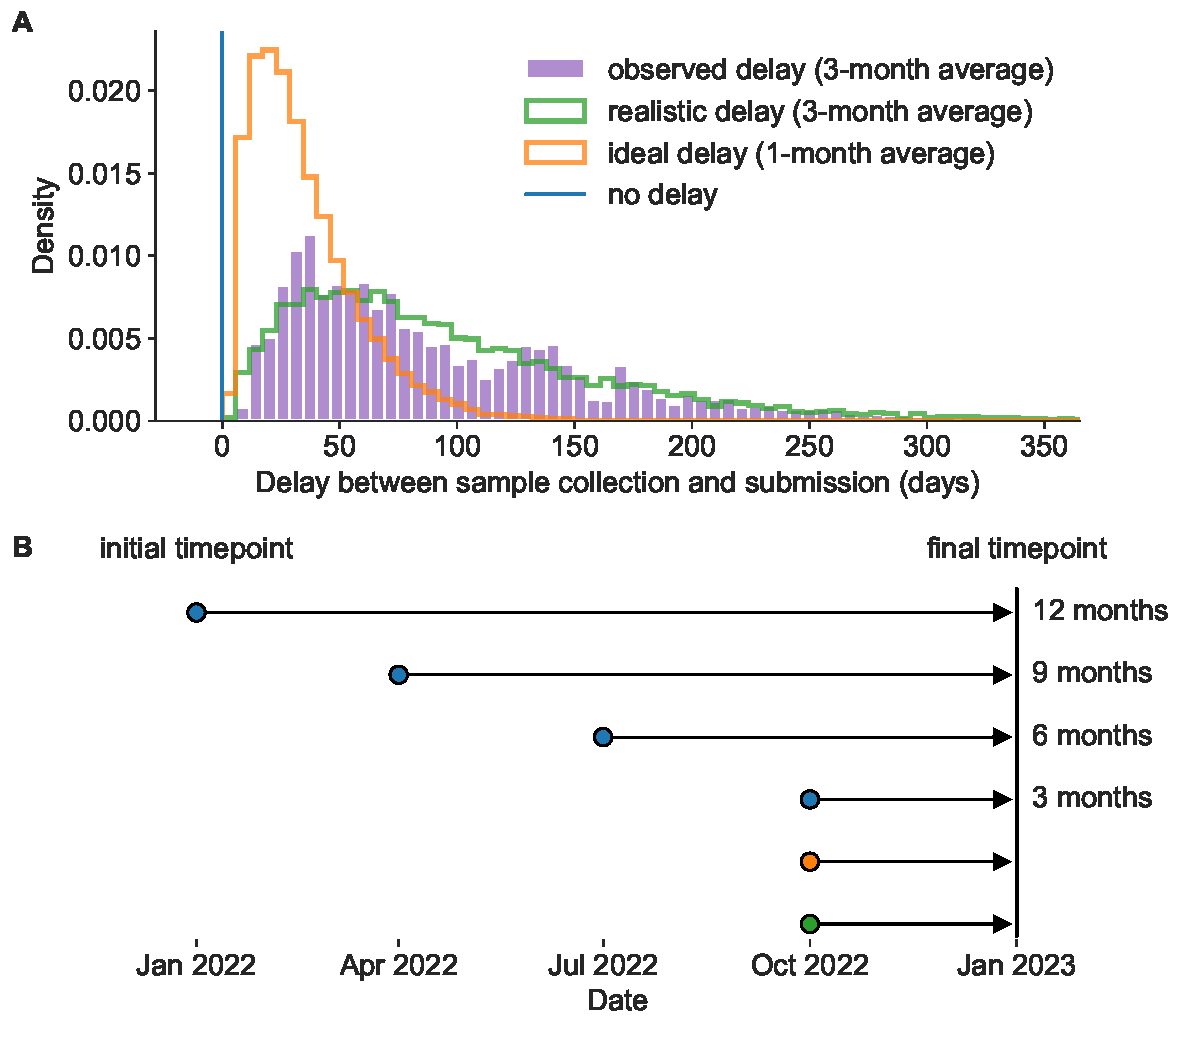
\includegraphics[width=\linewidth]{figures/distribution_of_delays_and_horizons}
\caption{Model of forecast horizons and submission delays.
  A) Long-term forecasting models historically predicted 12 months into the future from April and October because of the time required to develop and distribute a new vaccine \citep{Luksza:2014hj}.
  We test three additional shorter forecast horizons in three-month intervals of 9, 6, and 3 months prior to the same time in the future season.
  For each forecast horizon, we calculate the accuracy of forecasts under each of the three submission delays reflected above including no delay (blue), realistic delay (green), and ideal delay (orange).
  B) Observed delays in days between collection of viral samples and submission of corresponding HA sequences to GISAID (purple) for samples collected in 2019 have a mean of 98 days (approximately 3 months).
  A gamma distribution fit to the observed delay distribution with a similar mean and shape (green) represents a realistic submission delay that we sample from to assign ``submission dates'' to simulated and natural H3N2 populations.
  A gamma distribution with a mean that is one third of the realistic distribution (orange) represents an ideal submission delay analogous to the 1-month average observed delays for SARS-CoV-2 genomes.
  Retrospective analyses including fitting of forecasting models typically filter HA sequences by collection date instead of submission dates in which case there is no delay (blue).
}\label{fig:model_of_delays_and_horizons}
%
\figsupp[Distribution of submission delays in days for the pre-pandemic era (2019-2020) and pandemic era (2022-2023)]
{Distribution of submission delays in days for the pre-pandemic era (2019-2020 in blue) and pandemic era (2022-2023 in orange).
  Vertical dashed lines represent mean delays for each distribution.
  \figsuppdata{Distribution of submission delays; see \url{https://doi.org/xxx}}}
{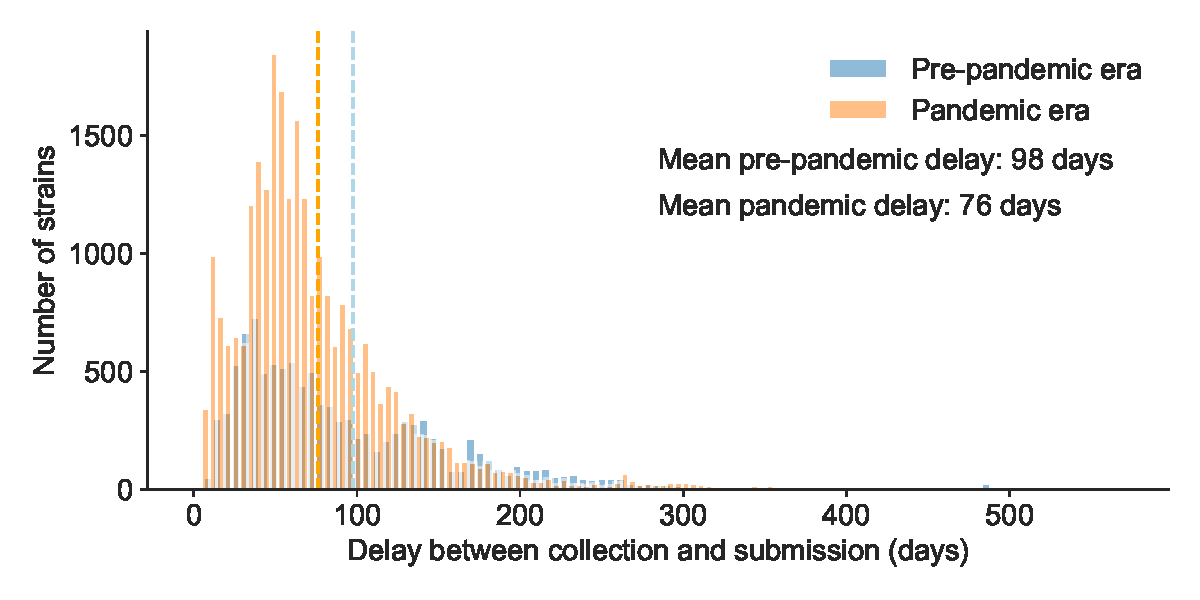
\includegraphics[width=6cm]{figures/distribution_of_delays_by_pandemic_era}}\label{figsupp:distribution_of_delays_by_pandemic_era}
%
\figsupp[Number and proportion of H3N2 sequences available per timepoint and delay type]
{
  A) Number of H3N2 sequences available per timepoint and delay type.
  B) Proportion of all H3N2 sequences without delay per timepoint and delay type.
}
{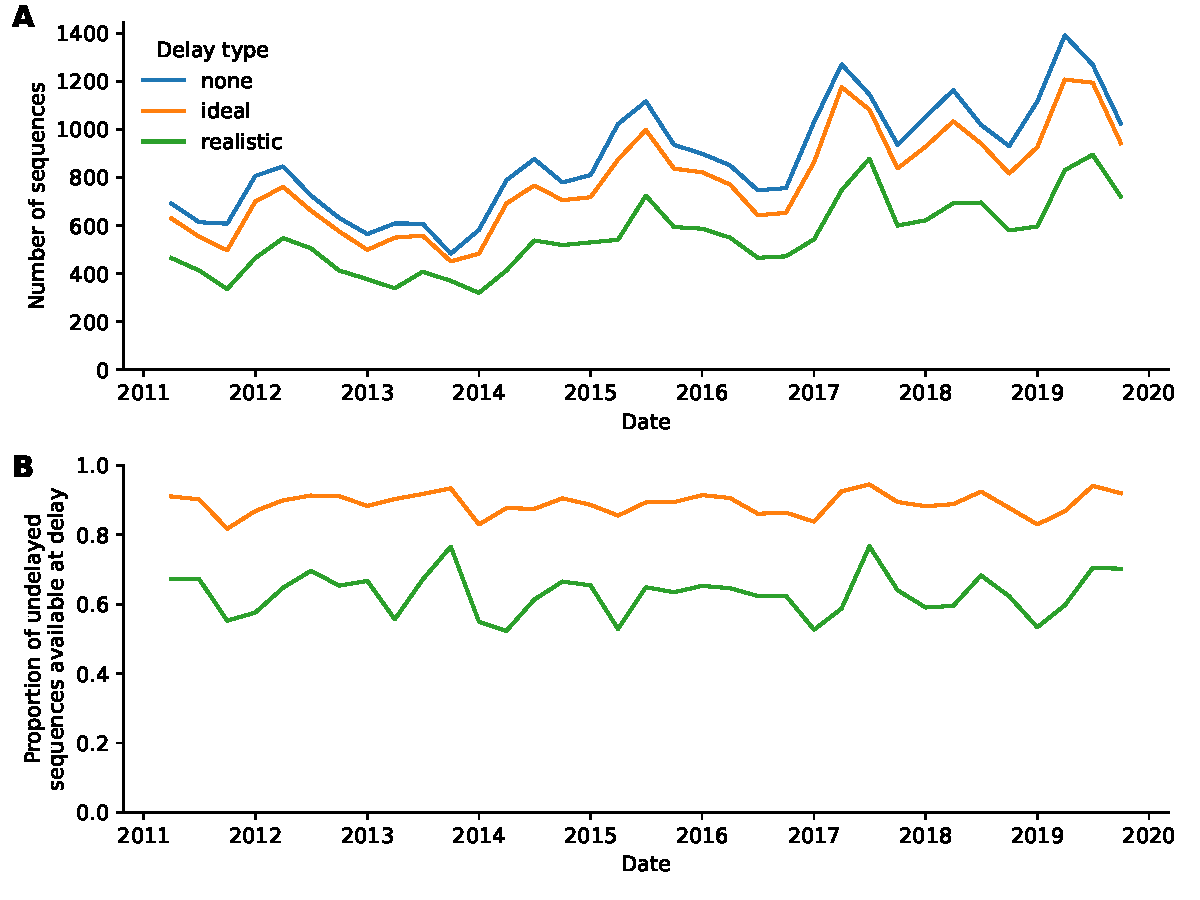
\includegraphics[width=6cm]{figures/h3n2_distribution_of_sequences_per_timepoint_and_delay}}\label{figsupp:distribution_of_h3n2_sequences_per_timepoint_and_delay}
%
\figsupp[Number and proportion of simulated H3N2-like sequences available per timepoint and delay type]
{
  A) Number of simulated H3N2-like sequences available per timepoint and delay type.
  B) Proportion of all simulated H3N2-like sequences without delay per timepoint and delay type.
}
{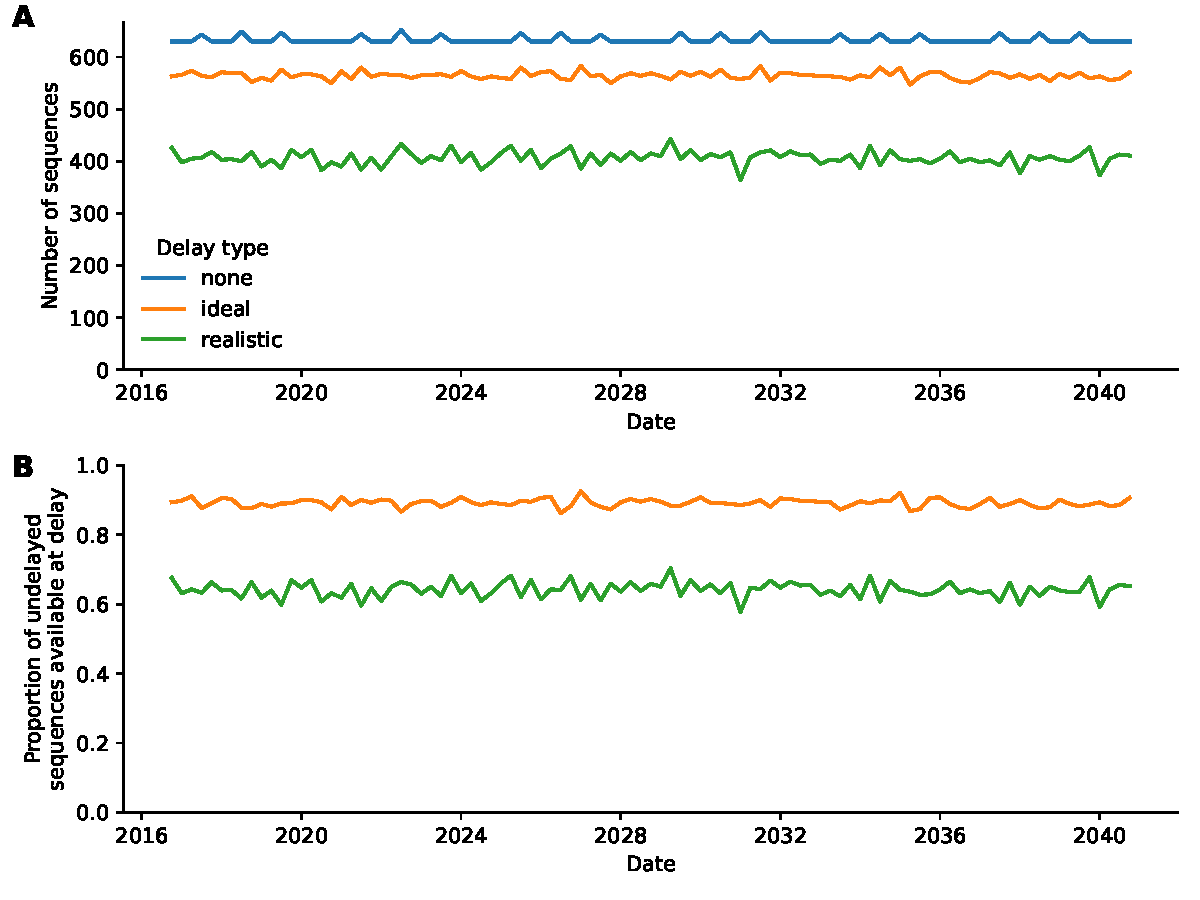
\includegraphics[width=6cm]{figures/simulated_distribution_of_sequences_per_timepoint_and_delay}}\label{figsupp:distribution_of_simulated_sequences_per_timepoint_and_delay}
\end{figure}

\section{Results}

\subsection{Reducing forecast horizons and submission delays decreases distances between predicted and observed future populations}

Previously, we trained long-term forecasting models that minimized the genetic distance between predicted and observed future populations of HA sequences \citep{Huddleston2020}.
We predicted each future population by projecting the frequency of each HA sequence from the initial population 12 months in the future based on the estimated fitness per sequence.
We calculated the distance between the frequencies and HA amino acid sequences of the predicted and observed future populations using the earth mover's distance metric \citep{Rubner1998}.
This metric provided an average distance between amino acid sequences of the two populations, allowing us to measure forecasting accuracy without prior clade definitions that could borrow information from the future or change between initial and future timepoints.
We identified the best forecasting models as those that minimized this distance between populations.
The most accurate sequence-only model for the 12-month forecast horizon estimated fitness with local branching index (LBI) \citep{Neher:2014eu} and mutational load \citep{Luksza:2014hj}.

To understand the effects of reducing forecast horizons and submission delays on long-term forecast accuracy, we produced forecasts 3, 6, 9, and 12 months into the future using HA sequences available at each initial timepoint under each submission delay scenario including no delay, ideal delay ($\sim$1-month average), and realistic delay ($\sim$3-month average) (\FIG{model_of_delays_and_horizons}, \FIGSUPP[model_of_delays_and_horizons]{distribution_of_h3n2_sequences_per_timepoint_and_delay}, \FIGSUPP[model_of_delays_and_horizons]{distribution_of_simulated_sequences_per_timepoint_and_delay}).
For natural A/H3N2 populations, we used the best sequence-only forecasting model, LBI and mutational load, which we previously trained on 12-month forecasts without any submission delay.
For simulated A/H3N2-like populations, we used the observed fitness per sample provided by the simulator.
For each forecast horizon and submission delay type, we calculated the earth mover's distance between the predicted future populations under the given delay scenario and the observed future populations without any delay in sequence availability.
We anticipated that reducing either the forecast horizon or the submission delay would reduce the distance to the future in amino acids (AAs), representing increased accuracy of the forecasting models.

We found that reducing the forecast horizon from the current standard of 12 months linearly reduced the distance to the future population predicted by the LBI and mutational load model (\FIG{h3n2_distances_to_the_future}).
Under the all three submission delay scenarios, the distance to the future reduced by approximately 1 AA on average for each 3-month reduction in forecast horizon (\TABLE{h3n2_distances_to_the_future}).
We observed the greatest average reduction in distance to the future ($\sim$1.4 AAs) between the 6- and 3-month forecast horizons.
Reducing the forecast horizon also noticeably reduced the variance per timepoint in predicted future populations across all delay scenarios (\FIG{h3n2_distances_to_the_future}).
For example, the standard deviation of distances to the future reduced from $\sim$2.6 AAs at the 12-month horizon to $\sim$1 AA at the 3-month horizon (\TABLE{h3n2_distances_to_the_future}).
We observed the same pattern for simulated A/H3N2-like populations (\FIGSUPP[h3n2_distances_to_the_future]{simulated_distances_to_the_future}).
Thus, reducing how far we have to predict into the future increased both forecast accuracy and precision.

\begin{figure}[htb]
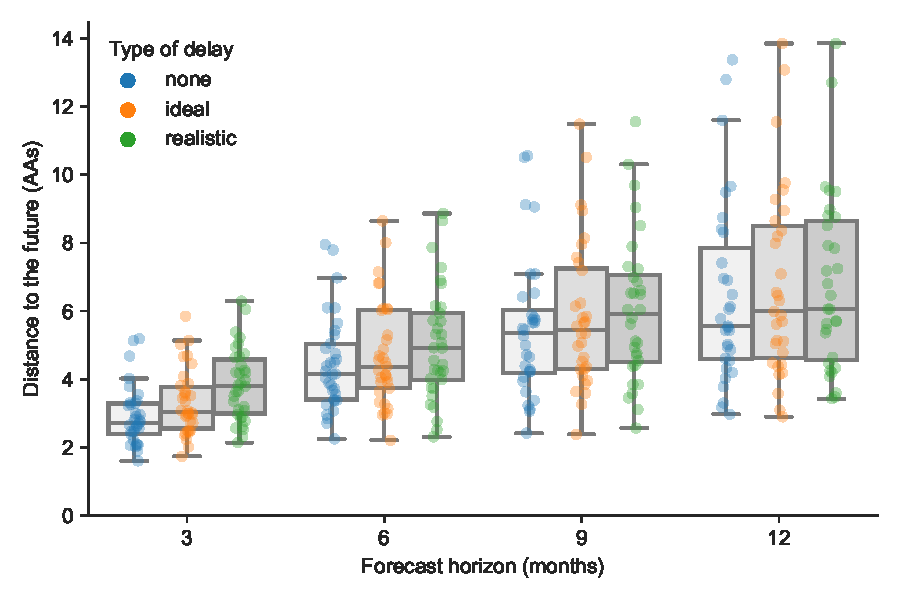
\includegraphics[width=\linewidth]{figures/h3n2_distances_to_the_future_by_delay_and_horizon}
\caption{Distance to the future per timepoint (AAs) for natural A/H3N2 populations by forecast horizon and submission delay type based on forecasts from the local branching index (LBI) and mutational load model.
  Each point represents a future timepoint whose population was predicted from the number of months earlier corresponding to the forecast horizon.
  Points are colored by submission delay type including forecasts made with no delay (blue), an ideal delay (orange), and a realistic delay (green).}
\label{fig:h3n2_distances_to_the_future}
%
\figsupp[Distance to the future for simulated H3N2-like populations]
{Distance to the future per timepoint (AAs) for simulated H3N2-like populations by forecast horizon and submission delay type.
  \figsuppdata{Distance to the future for simulated H3N2-like populations; see \url{https://doi.org/xxx}}}
{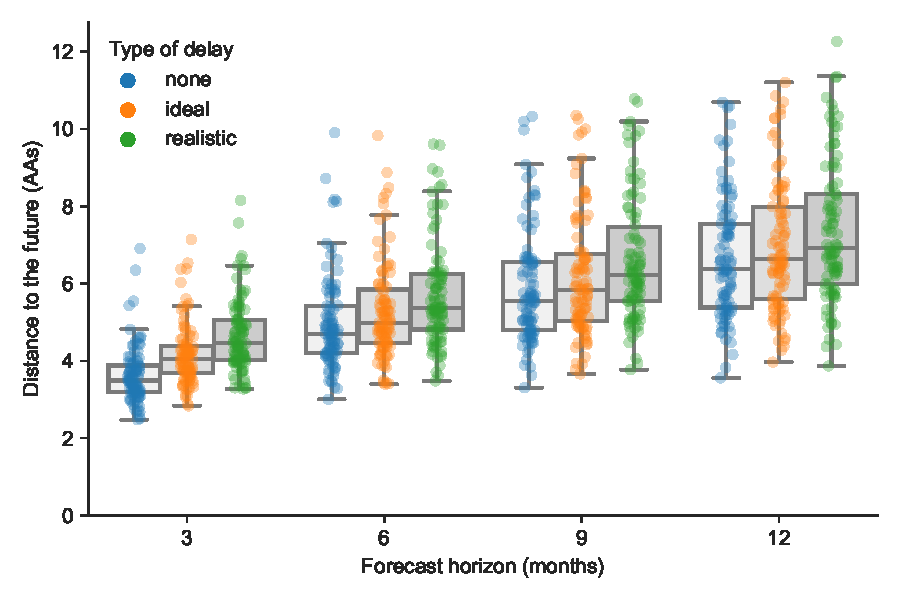
\includegraphics[width=6cm]{figures/simulated_distances_to_the_future_by_delay_and_horizon}}\label{figsupp:simulated_distances_to_the_future}
%
\figdata{Distance to the future for natural H3N2 populations.}\label{figdata:h3n2_distances_to_the_future}
\figsrccode{Jupyter notebook used to produce this figure and the supplemental figure lives in \texttt{workflow/notebooks/plot-distances-to-the-future-by-delay-type-and-horizon-for-population.py.ipynb}.}\label{figsrccode:distances_to_the_future}
\end{figure}

\begin{table}[htb]
  \begin{center}
    
\begin{tabular*}{0.7\textwidth}{rrrr}
\toprule
          & \multicolumn{3}{c}{Distance to future (mean +/- std dev AAs)} \\
  Horizon & No delay & Ideal delay & Realistic delay \\
\midrule

3 & 2.91 +/- 0.86 & 3.32 +/- 0.96 & 3.85 +/- 1.05 \\
6 & 4.44 +/- 1.39 & 4.74 +/- 1.54 & 5.03 +/- 1.66 \\
9 & 5.48 +/- 2.05 & 5.84 +/- 2.14 & 6.04 +/- 2.15 \\
12 & 6.45 +/- 2.72 & 6.77 +/- 2.80 & 6.78 +/- 2.61 \\

\bottomrule
\end{tabular*}


    \caption{Distance to the future in amino acids (mean +/- standard deviation AAs) by forecast horizon (in months) and submission delay for H3N2 populations.}
    \label{tab:h3n2_distances_to_the_future}
  \end{center}
\end{table}

In contrast, we found that reducing submission delays from a $\sim$3-month average delay in the realistic scenario to a $\sim$1-month average delay in the ideal scenario had a weaker effect on distance to the future.
At the 12-month forecast horizon, the ideal and realistic delay scenarios produced similar predictions, with the only noticeable improvement observed under the scenario without any submission delays (\FIG{h3n2_distances_to_the_future}).
As the forecast horizon decreased, the effect of submission delays appeared more prominent, with the greatest effect of reduced delays observed at the 3-month forecast horizon.
However, the average improvement from the realistic to the ideal submission delay scenario at the 3-month horizon was still only $~\sim$0.3 AAs (\TABLE{h3n2_distances_to_the_future}).
Reducing submission delays also had little effect on the variance per timepoint in predicted future populations.
Interestingly, we observed a stronger effect of reducing submission delays in simulated A/H3N2-like populations, with the best average improvement between realistic and ideal delays of $\sim$0.7 AAs at the 3-month horizon (\FIGSUPP[h3n2_distances_to_the_future]{simulated_distances_to_the_future}).
As with natural A/H3N2 populations, the effect of reducing submission delays appeared to increase as the forecast horizon decreased.
These results indicate that reducing submission delays may have little effect under the current 12-month forecast approach used for influenza vaccine composition, but reducing submission delays should become increasingly important as we forecast from closer to future influenza populations.

\subsection{Reducing submission delays improves estimates of current clade frequencies}

Although the distance between predicted and observed future populations in amino acids provides an unbiased metric to optimize forecasting models, in practice, we use these models to forecast clade frequencies.
We predict each clade's future frequency as the sum of the initial frequency times the estimated fitness for each HA sequence in the clade.
Given the importance of initial clade frequencies in these forecasts, we tested the effect of submission delays on current clade frequency estimates.
For each timepoint and clade with a frequency greater than zero under the scenario without delays, we calculated the clade frequency error as the difference between clade frequency without submission delays and the frequency with either an ideal or realistic delay.
Positive error values represented underestimation of current clades, while negative values represented overestimation.

Across all clade frequencies, we found that errors in current clade frequencies for H3N2 appeared normally distributed with lower variance in the ideal delay scenario than under realistic delays (\FIG{h3n2_current_clade_frequency_errors}A and B).
Of the 822 clades under the scenario without delays, 613 (75\%) had a frequency less than 10\%, representing small, emerging clades.
The remaining 209 (25\%) had a frequency of 10\% or greater, representing larger clades that could be more likely to succeed.
To understand whether delays had different effects on these small and large clades, respectively, we inspected clades from these latter two groups separately.
For small clades, errors under ideal delays ranged from -4\% to 4\% with a standard deviation of 1\%, while realistic delays produced errors ranging from -8\% to 7\% with a standard deviation of 2\% (\FIG{h3n2_current_clade_frequency_errors}C).
We did not observe a bias toward underestimation or overestimation of initial small clade frequencies under either delay scenario.
For large clades, errors under ideal delay ranged from -9\% to 14\% with a standard deviation of 3\% (\FIG{h3n2_current_clade_frequency_errors}D).
Errors under realistic delays ranged from -16\% to 29\% with a standard deviation of 6\%.
We observed a slight bias toward underestimation of large clades under the realistic delay scenario, with a median error of 1\%.
These results show that reducing submission delays for natural H3N2 populations from a 3-month average to a 1-month average could reduce the bias toward underestimated large clade frequencies and reduce the standard deviation of all current clade frequency errors by 50\%.

\begin{figure}[htb!]
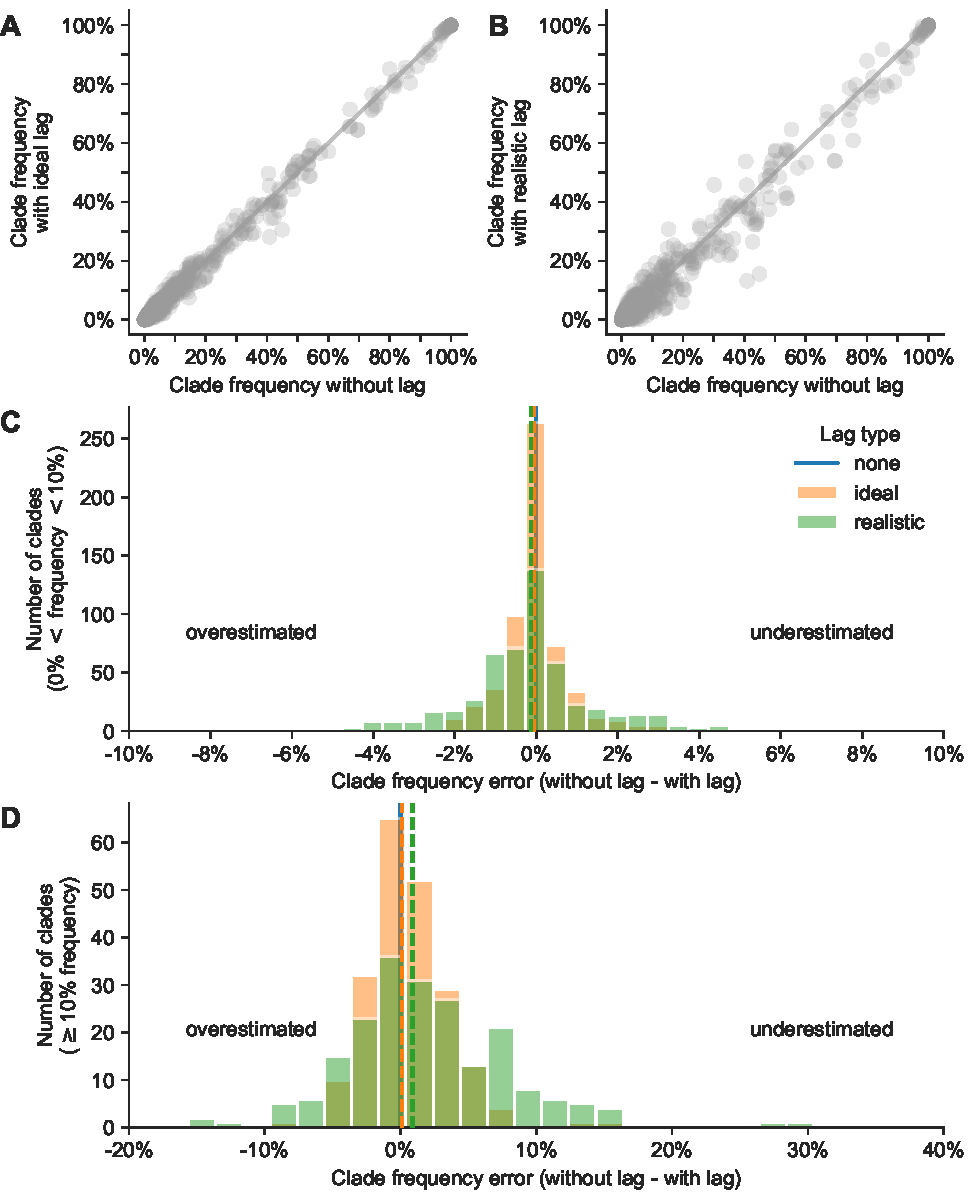
\includegraphics[width=\linewidth]{figures/h3n2_current_frequency_errors_by_delay}
\caption{Clade frequency errors for natural A/H3N2 clades at the same timepoint calculated as the difference between clade frequencies without submission delay and corresponding frequencies with either A) ideal or B) realistic submission delays.
Distributions of frequency errors appear normally distributed in both delay scenarios for both C) small clades ($>$0\% and $<$10\% frequency) and D) large clades ($\ge$10\%).
Dashed lines indicate the median error from the distribution of the delay type with the same color.}
\label{fig:h3n2_current_clade_frequency_errors}
%
\figsupp[Current clade frequency errors for simulated H3N2-like populations]
{Clade frequency errors between simulated H3N2-like HA populations with ideal or realistic submission delays and populations without any submission delay.
  \figsuppdata{Current frequencies per sequence in each simulated H3N2-like tree of the forecast analysis by delay type (none, ideal, and realistic); see \url{https://doi.org/xxx}}}
{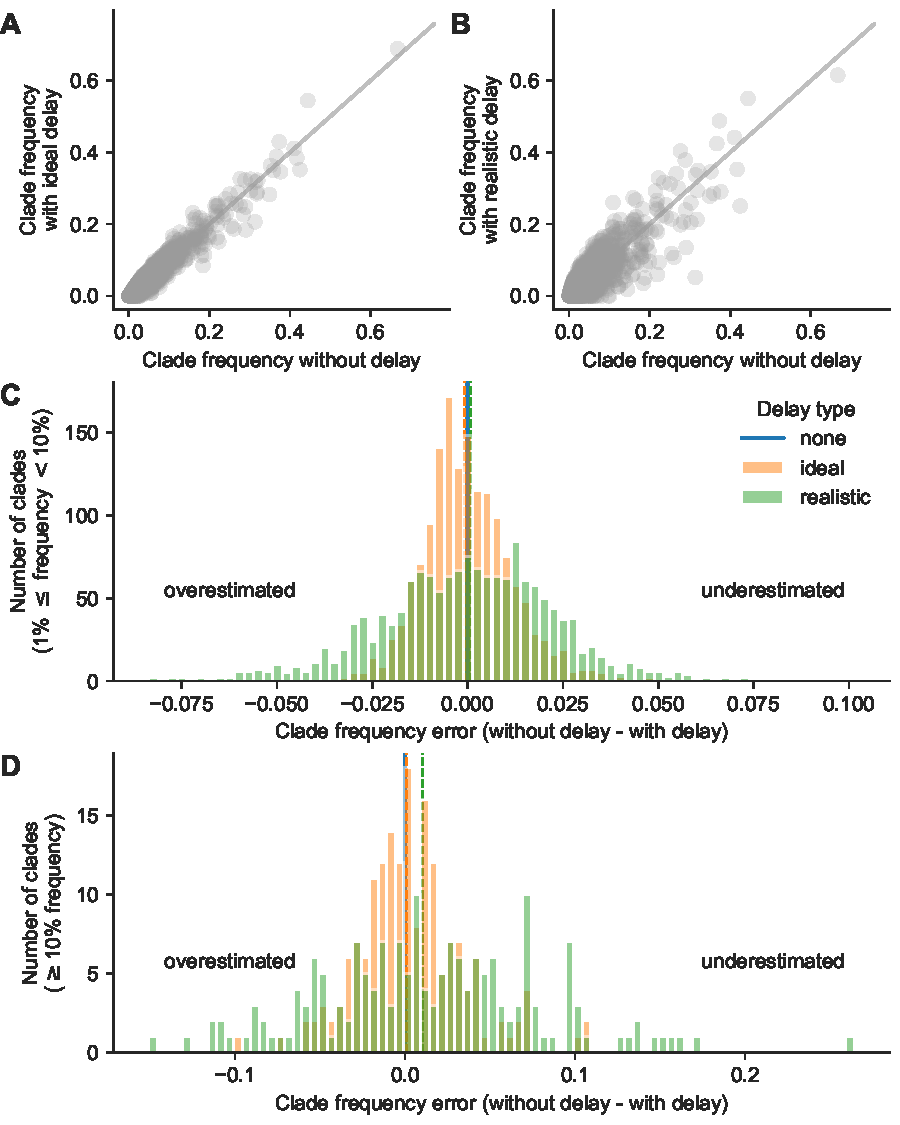
\includegraphics[width=6cm]{figures/simulated_current_frequency_errors_by_delay}}\label{figsupp:simulated_current_clade_frequency_errors}
%
\figdata{Current frequencies per sequence in each natural H3N2 tree of the forecast analysis by delay type (none, ideal, and observed).}\label{figdata:h3n2_tip_attributes}
\figsrccode{Jupyter notebook used to produce this figure and the supplemental figure lives in \texttt{workflow/notebooks/plot-current-clade-frequency-errors-by-delay-type-for-populations.py.ipynb}.}\label{figsrccode:current_clade_frequency_errors}
\end{figure}

Delayed submissions similarly affected clade frequencies for simulated A/H3N2-like populations (\FIGSUPP[h3n2_current_clade_frequency_errors]{simulated_current_clade_frequency_errors}).
Small clade errors under ideal delays ranged from -4\% to 6\% (standard deviation of 1\%) and under realistic delays ranged from -9\% to 8\% (standard deviation of 2\%) (\FIGSUPP[h3n2_current_clade_frequency_errors]{simulated_current_clade_frequency_errors}C).
For large clades, errors under ideal delays ranged from -8\% to 18\% (standard deviation of 3\%) and under realistic delays from -14\% to 40\% (standard deviation of 7\%) (\FIGSUPP[h3n2_current_clade_frequency_errors]{simulated_current_clade_frequency_errors}D).
As with natural H3N2 populations, we observed a slight bias in simulated populations under realistic delays toward underestimation of large clade frequencies with a median error of 2\%.
We also observed a similar reduction in standard deviation of current frequency errors for these simulated H3N2-like populations when switching from realistic to ideal submission delays.

\subsection{Reducing forecast horizons increases the accuracy and precision of clade frequency forecasts}

Next, we estimated the effects of different forecast horizons and submission delays on the accuracy of clade frequency forecasts.
For this analysis, we focused on larger clades with an initial frequency $\ge$10\% which represent more established clades that would appear in biannual reports to the WHO's vaccine composition meetings \citep{Huddleston2024}.
For each combination of initial timepoint, future timepoint, and delay scenario (\FIG{model_of_delays_and_horizons}A), we calculated initial and predicted future frequencies for all clades present under the given delay and then calculated the corresponding observed future frequencies without delay for clades that descended from the clades present at the initial timepoint.
We calculated the error in forecast frequencies as the difference between predicted future frequencies under the given delay scenario and observed future frequencies without any delay.

As with current clade frequency errors, forecast clade frequency errors appeared to be normally distributed (\FIG{h3n2_forecast_clade_frequency_errors}).
This pattern matched our expectation that at any given initial timepoint the overestimation of one clade's future frequency must cause an underestimation of another current clade's future frequency.
The standard deviation of forecast errors decreased with decreasing forecast horizon and, with the exception of the 12-month horizon, with decreasing submission delays (\TABLE{h3n2_forecast_clade_frequency_errors}).
Reducing the forecast horizon had a greater effect on the variation in forecast errors than reducing submission delays.
For example, the standard deviation of forecast errors at the 12-month horizon under realistic submission delays was 30\%, while the standard deviation for the 6-month horizon under realistic delays was 17\% (\TABLE{h3n2_forecast_clade_frequency_errors}).
In contrast, the standard deviation at the 12-month horizon under ideal submission delays was slightly higher at 32\%.
For all other forecast horizons, reducing the submission delays from realistic to ideal only reduced the standard deviation by 1\%.
We found similar patterns for the absolute values of forecast clade frequency errors where reducing the forecast horizon from 12 months to 6 reduced the average absolute error from 24\% to 15\%, but reducing the submission delays under any forecast horizon had little effect (\TABLE{h3n2_forecast_clade_frequency_errors}).
These results show that the effect size of submission delays on forecast errors is low relative to the effect of the forecast horizon.

\begin{figure}[htb]
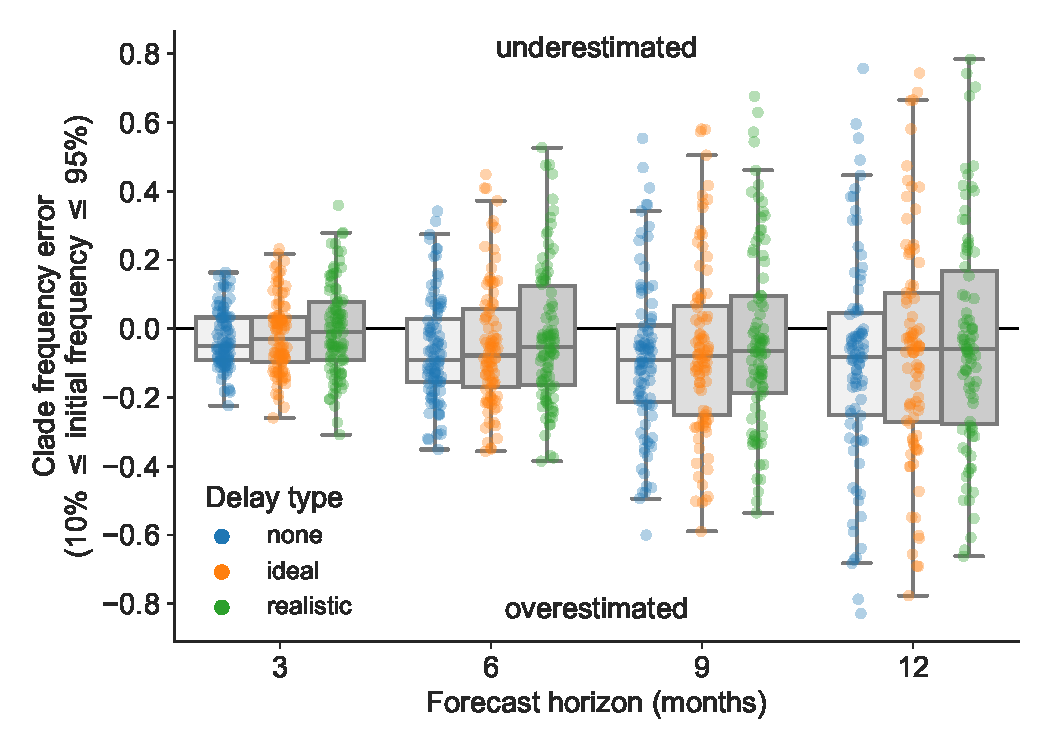
\includegraphics[width=\linewidth]{figures/h3n2_forecast_frequency_errors_by_delay_and_horizon}
\caption{Forecast clade frequency errors for natural H3N2 populations by forecast horizon in months and submission delay type (none, ideal, or observed).}
\label{fig:h3n2_forecast_clade_frequency_errors}
%
\figsupp[Forecast clade frequency errors for simulated H3N2-like populations.]
{Forecast clade frequency errors for simulated H3N2-like HA populations by forecast horizon in months and submission delay type (none, ideal, or realistic).
  \figsuppdata{Current, predicted future, and observed future clade frequencies per initial timepoint, forecast horizon, and submission delay type for simulated H3N2-like populations; see \url{https://doi.org/xxx}}}
{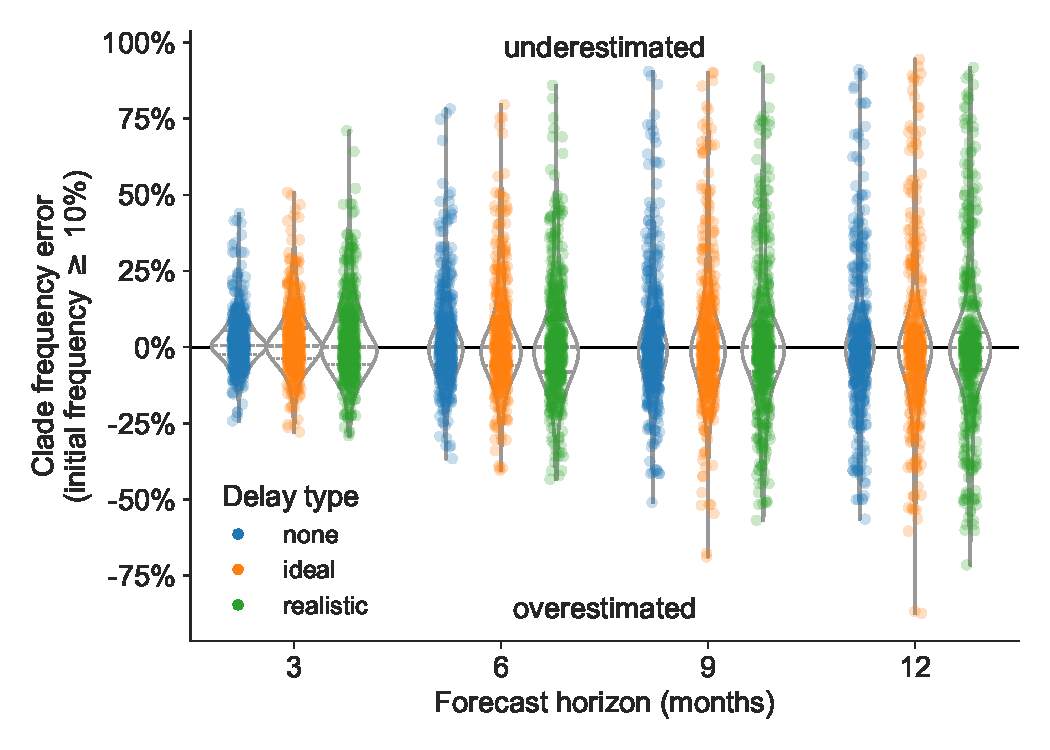
\includegraphics[width=6cm]{figures/simulated_forecast_frequency_errors_by_delay_and_horizon}}\label{figsupp:simulated_forecast_clade_frequency_errors}
%
\figdata{Current, predicted future, and observed future clade frequencies per initial timepoint, forecast horizon, and submission delay type for H3N2 populations.}\label{figdata:h3n2_clade_frequencies}
\figsrccode{Jupyter notebook used to produce this figure and the supplemental figures lives in \texttt{workflow/notebooks/plot-forecast-clade-frequency-errors-by-delay-type-and-horizon-for-population.py.ipynb}.}\label{figsrccode:forecast_clade_frequency_errors}
\end{figure}

We observed a slight but consistent bias toward the overestimation of future clade frequencies with median errors ranging from -5\% to -10\% across all forecast horizons and submission delays (\FIG{h3n2_forecast_clade_frequency_errors} and \TABLE{h3n2_forecast_clade_frequency_errors}).
Although the average absolute clade frequency error consistently decreased with decreasing forecast horizon, we did not see the same decrease in the average clade frequency error except at a forecast horizon of 3 months (\TABLE{h3n2_forecast_clade_frequency_errors}).
We observed the same pattern in simulated H3N2-like populations (\FIGSUPP[h3n2_forecast_clade_frequency_errors]{simulated_forecast_clade_frequency_errors}).
Since this pattern of overestimation appeared in both natural and simulated populations even without submission delays, overestimation may be a feature of the forecasting framework itself rather than a feature of the different viral populations or fitness metrics.
To better understand this pattern, we investigated the relationship between forecast errors and initial clade frequencies across forecast horizons and delays.
These results suggest that larger clades with overestimated initial frequencies partially contribute to the observed bias toward overestimating forecast clade frequencies.
However, we attributed the majority of this pattern to the limitations of predicting the future frequencies of large clades circulating at a given time when extant smaller clades are likely to grow during the period of the forecast horizon.

\begin{table}[htb]
  \begin{center}
    
\begin{tabular*}{1.0\textwidth}{rrrrrrrrrr}
\toprule
        &            & \multicolumn{5}{c}{Clade frequency error (\%)} & \multicolumn{3}{c}{Absolute frequency error (\%)} \\
Horizon & Delay type & Mean & Median & Std Dev & Min & Max & Mean & Median & Std Dev \\
\midrule

3 & none & 1 & 0 & 9 & -28 & 28 & 7 & 6 & 6 \\
3 & ideal & 1 & 0 & 11 & -32 & 36 & 8 & 6 & 7 \\
3 & realistic & 1 & 0 & 13 & -31 & 50 & 10 & 7 & 9 \\
6 & none & 1 & 0 & 17 & -48 & 45 & 12 & 9 & 11 \\
6 & ideal & 1 & 0 & 19 & -50 & 53 & 13 & 9 & 13 \\
6 & realistic & 1 & 0 & 20 & -52 & 75 & 15 & 12 & 14 \\
9 & none & 0 & -1 & 23 & -66 & 59 & 16 & 10 & 17 \\
9 & ideal & 1 & -1 & 25 & -67 & 58 & 18 & 11 & 18 \\
9 & realistic & 1 & -1 & 26 & -67 & 79 & 19 & 12 & 19 \\
12 & none & 0 & 0 & 30 & -82 & 76 & 20 & 10 & 22 \\
12 & ideal & 1 & 0 & 31 & -80 & 74 & 21 & 9 & 23 \\
12 & realistic & 0 & 0 & 31 & -78 & 78 & 20 & 12 & 23 \\

\bottomrule
\end{tabular*}


    \caption{Errors in clade frequencies between observed and predicted values by forecast horizon (in months) and submission delay for H3N2 clades with an initial frequency $\geq$10\% under the given delay scenario.}
    \label{tab:h3n2_forecast_clade_frequency_errors}
  \end{center}
\end{table}

\subsection{Reduced vaccine development time provides the best improvement in forecast accuracy of available realistic interventions}

Although we have investigated the effects of a range of forecast horizons and submission delays, not all of these scenarios are currently realistic.
The most we can hope to reduce the forecast horizon with current mRNA vaccine technology is from 12 months to 6 months and the most we could reduce submission delays would be from an average of 3 months to 1 month \citep{Grant2023}.
In practice, we wanted to know how much a reduction in forecast horizon or submission delay could improve the accuracy of forecasts to each future timepoint.
To determine the effects of realistic interventions on forecast accuracy, we inspected the reduction in total absolute forecast error per future timepoint associated with improved vaccine development (reducing forecast horizon from 12 months to 6 months), improved genomic surveillance (reducing delays from a 3-month average to 1 month), and the combination of both improvements.
We selected all forecasts with a 12-month horizon and a realistic delay, to represent current forecast conditions or ``the status quo''.
Then, we selected forecasts for the same future timepoints present in the current conditions for a 6-month horizon and a realistic delay, a 12-month horizon and an ideal delay, and 6-month horizon and an ideal delay.
Since forecasts between different initial and future timepoints could be represented by different clades, we could not compare forecasts for specific clades between interventions.
Instead, we calculated the total absolute clade frequency error per future timepoint under each intervention and calculated the improvement in forecast accuracy as the difference in total error between the current conditions and each intervention.
In addition to this clade-based analysis, we also estimated improvement in forecast accuracy by the difference in distance to the future between different scenarios.
For both analyses, positive values represented improved forecast accuracy under a given intervention scenario and negative values represented a reduction in accuracy.

\begin{figure}[htb]
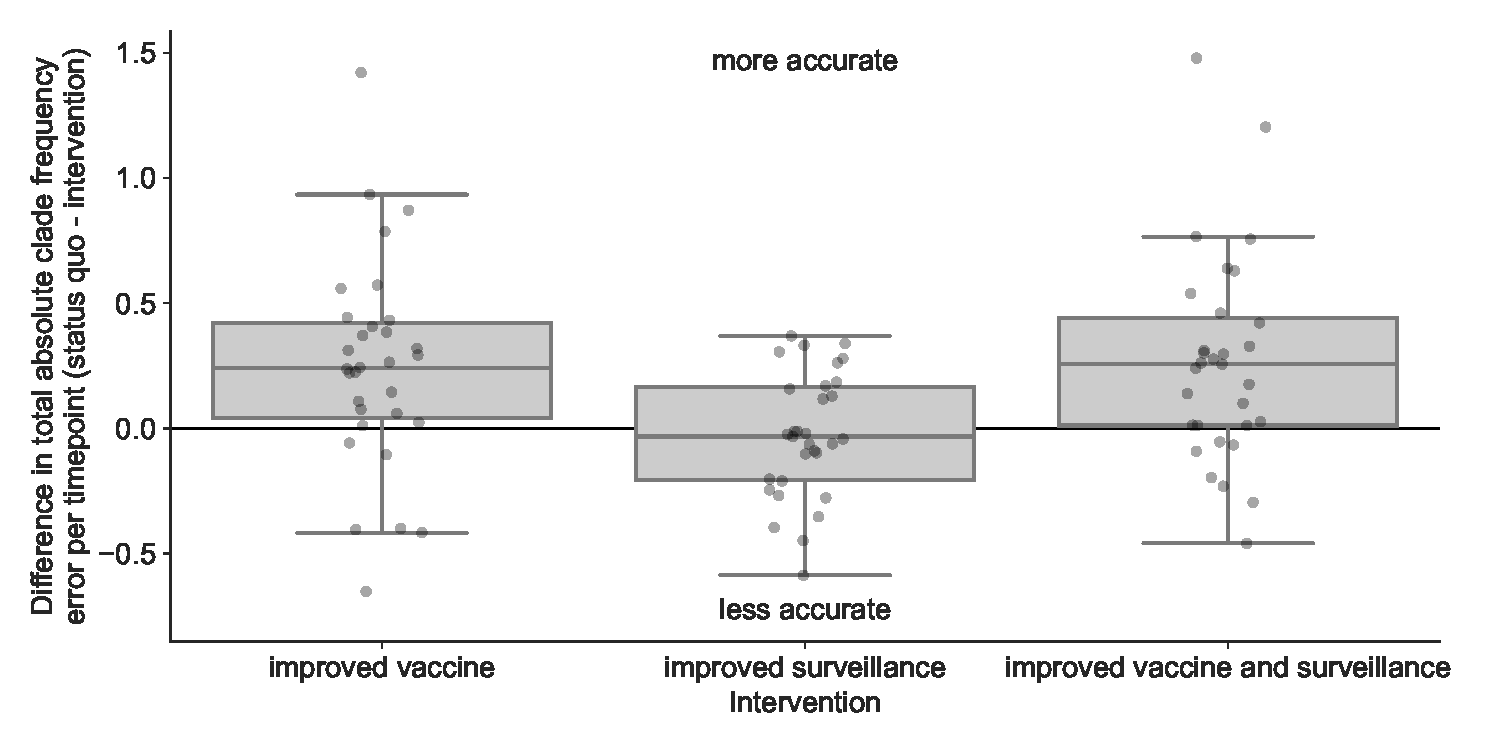
\includegraphics[width=\linewidth]{figures/h3n2_effects_of_realistic_interventions}
\caption{Improvement of clade frequency errors for H3N2 populations between the status quo (12-month forecast horizon and realistic submission delays) and realistic interventions.}
\label{fig:h3n2_effects_of_realistic_interventions}
%
\figsupp[Distribution of total absolute clade frequency errors summed across clades per future timepoint for H3N2 populations.]
{Distribution of total absolute clade frequency errors summed across clades per future timepoint for H3N2 populations.\
  We calculated the effects of interventions as the difference between these values per future timepoint under the status quo (12-month forecast horizon and realistic submission delay) and specific interventions.
  \figsuppdata{Total absolute clade frequency errors per future timepoint for H3N2 populations; see \url{https://doi.org/xxx}}}
{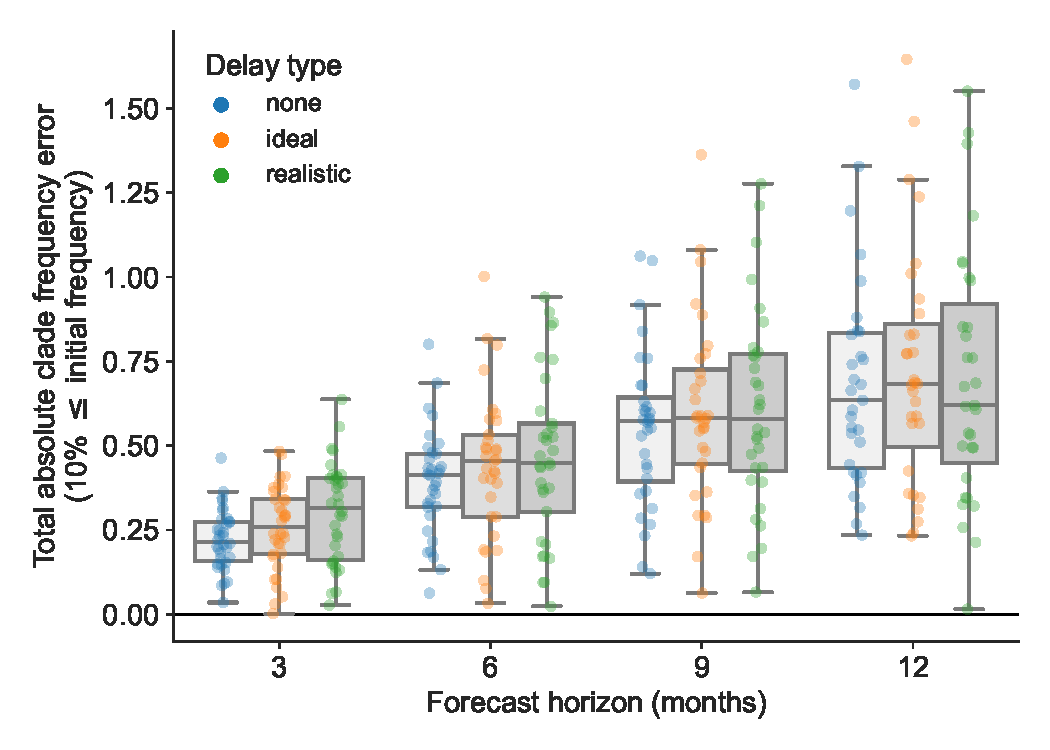
\includegraphics[width=6cm]{figures/h3n2_total_absolute_forecast_frequency_errors_by_delay_and_horizon}}\label{figsupp:h3n2_total_absolute_clade_frequency_errors}
%
\figsupp[Improvement of clade frequency errors for simulated H3N2-like populations.]
{Improvement of clade frequency errors for simulated H3N2-like populations between the status quo and realistic interventions.
  \figsuppdata{Differences in absolute clade frequency error per future timepoint and clade between the status quo and realistic interventions for simulated H3N2-like populations; see \url{https://doi.org/xxx}}}
{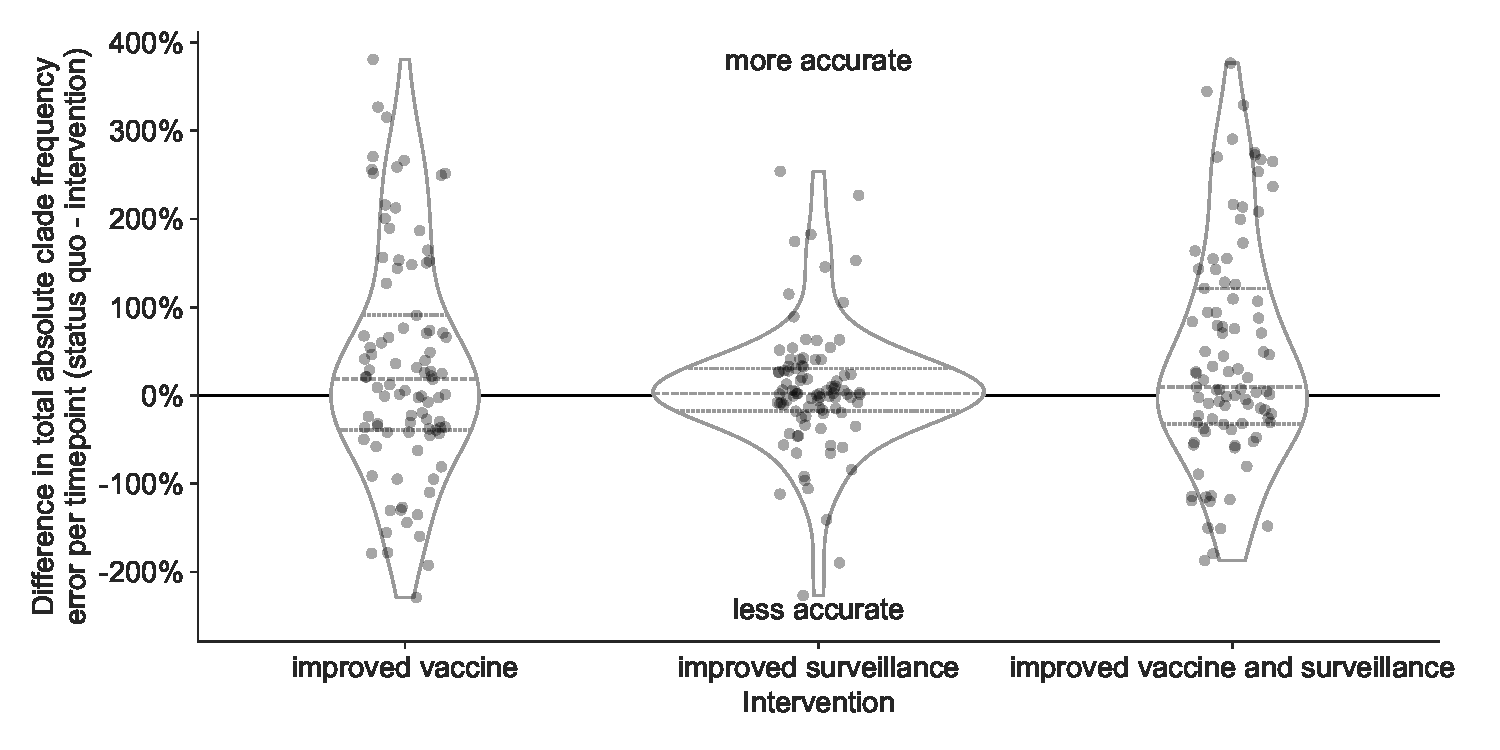
\includegraphics[width=6cm]{figures/simulated_effects_of_realistic_interventions}}\label{figsupp:simulated_effects_of_realistic_interventions}
%
\figsupp[Distribution of total absolute clade frequency errors summed across clades per future timepoint for simulated H3N2-like populations.]
{Distribution of total absolute clade frequency errors summed across clades per future timepoint for simulated H3N2-like populations.\
  \figsuppdata{Total absolute clade frequency errors per future timepoint for simulated H3N2-like populations; see \url{https://doi.org/xxx}}}
{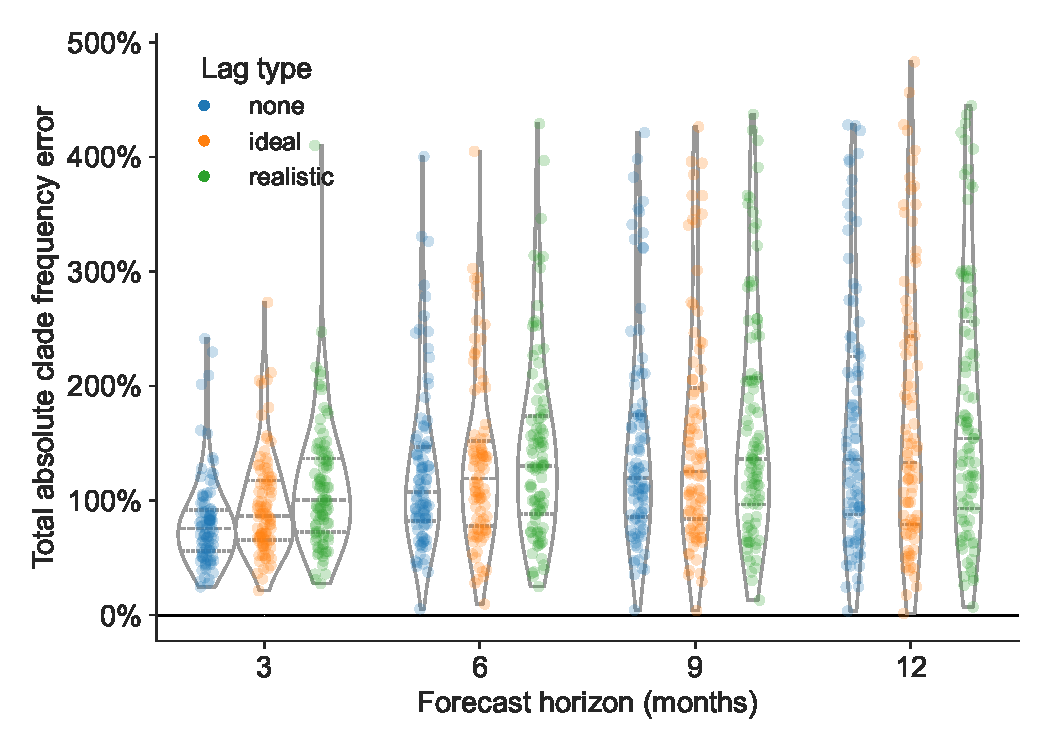
\includegraphics[width=6cm]{figures/simulated_total_absolute_forecast_frequency_errors_by_delay_and_horizon}}\label{figsupp:simulated_total_absolute_clade_frequency_errors}
%
\figsupp[Improvement of distances to the future (AAs) for H3N2 populations between the status quo (12-month forecast horizon and realistic submission delays) and realistic interventions.]
{Improvement of distances to the future (AAs) for H3N2 populations between the status quo (12-month forecast horizon and realistic submission delays) and realistic interventions.\
  The effects of interventions are the differences between distances to the future per future timepoint under the status quo and specific interventions.
  \figsuppdata{Improvement of distances to the future per future timepoint for H3N2 populations; see \url{https://doi.org/xxx}}}
{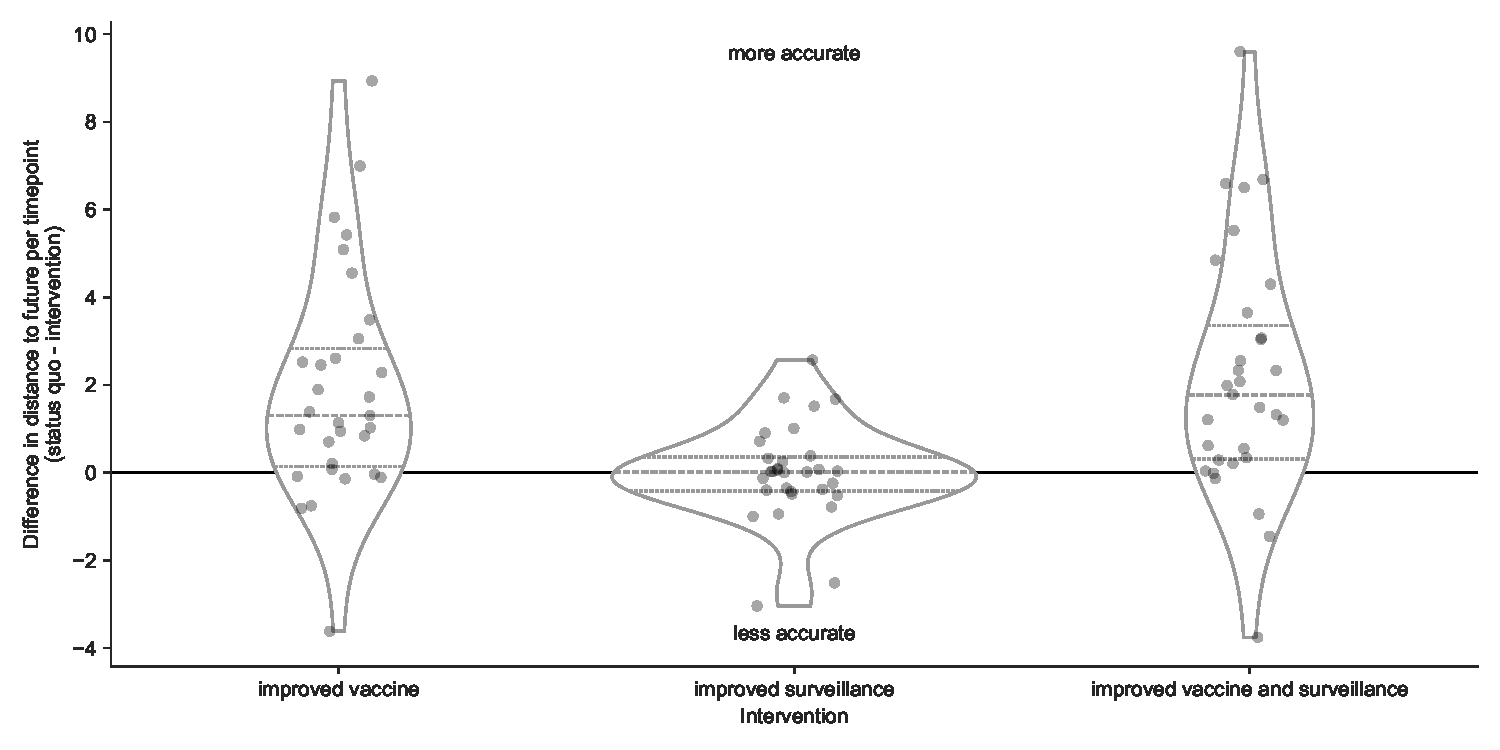
\includegraphics[width=6cm]{figures/h3n2_effects_of_realistic_interventions_on_distances_to_the_future}}\label{figsupp:h3n2_effects_of_realistic_interventions_on_distances_to_the_future}
%
\figsupp[Improvement of distances to the future (AAs) for simulated H3N2-like populations between the status quo (12-month forecast horizon and realistic submission delays) and realistic interventions.]
{Improvement of distances to the future (AAs) for simulated H3N2-like populations between the status quo (12-month forecast horizon and realistic submission delays) and realistic interventions.\
  The effects of interventions are the differences between distances to the future per future timepoint under the status quo and specific interventions.
  \figsuppdata{Improvement of distances to the future per future timepoint for simulated H3N2-like populations; see \url{https://doi.org/xxx}}}
{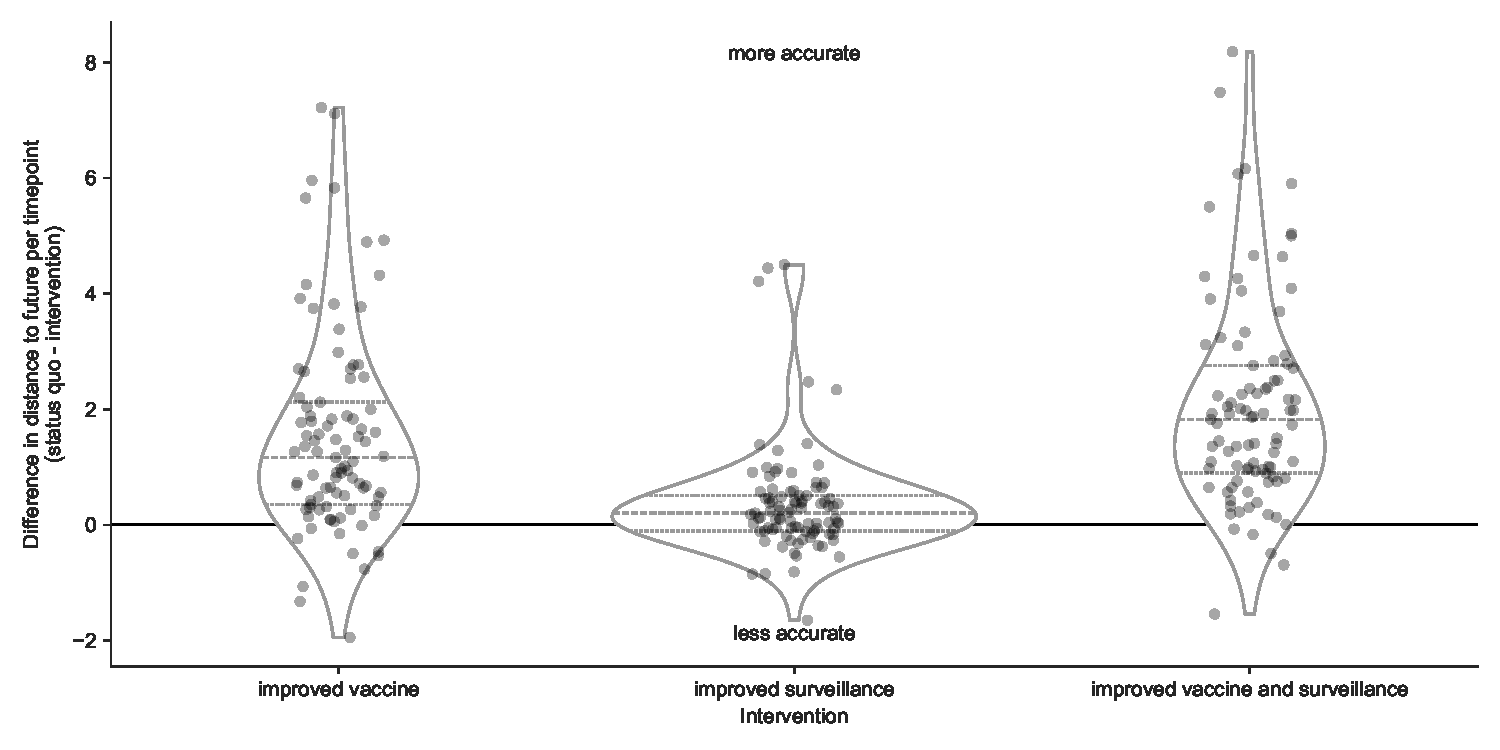
\includegraphics[width=6cm]{figures/simulated_effects_of_realistic_interventions_on_distances_to_the_future}}\label{figsupp:simulated_effects_of_realistic_interventions_on_distances_to_the_future}
%
\figdata{Differences in absolute clade frequency error per future timepoint and clade between the status quo and realistic interventions for H3N2 populations.}\label{figdata:h3n2_effects_of_realistic_interventions}
\figsrccode{Jupyter notebook used to produce effects of interventions on total absolute clade frequency errors \texttt{workflow/notebooks/plot-forecast-clade-frequency-errors-by-delay-type-and-horizon-for-population.py.ipynb}.}\label{figsrccode:effects_of_realistic_interventions}
\figsrccode{Jupyter notebook used to produce effects of interventions on distances to the future lives in \texttt{workflow/notebooks/plot-distances-to-the-future-by-delay-type-and-horizon-for-population.py.ipynb}.}\label{figsrccode:effects_of_realistic_interventions_on_distances_to_the_future}
\end{figure}

\begin{table}[htb]
  \begin{center}
    
\begin{tabular*}{1.0\textwidth}{rrrrrr}
\toprule
             & \multicolumn{3}{c}{Forecast accuracy improvement (\%)} & \multicolumn{2}{c}{Forecasts improved} \\
Intervention & Mean & Median & Std Dev & Total & Proportion \\
\midrule

improved vaccine & 32 & 33 & 46 & 23 & 0.74 \\
improved surveillance & -6 & -1 & 24 & 13 & 0.42 \\
improved vaccine and surveillance & 33 & 42 & 45 & 24 & 0.77 \\

\bottomrule
\end{tabular*}


    \caption{Improvement in H3N2 forecast accuracy under realistic interventions of improved vaccine development (reducing 12-month to 6-month forecast horizon), improved surveillance (reducing submission delays from 3 months on average to 1 month), or a combination of both interventions.
      We measured improvements from the status quo (12-month forecast horizon and 3-month average submission delay) as the difference in total absolute clade frequency error per future timepoint and the number and proportion of future timepoint forecasts that improved under the intervention.}
    \label{tab:h3n2_effects_of_realistic_interventions}
  \end{center}
\end{table}

Both interventions with improved vaccine development increased forecast accuracy for the majority of future timepoints (\FIG{h3n2_effects_of_realistic_interventions}, \TABLE{h3n2_effects_of_realistic_interventions}, and \FIGSUPP[h3n2_effects_of_realistic_interventions]{h3n2_total_absolute_clade_frequency_errors}).
In contrast, the intervention that only improved genomic surveillance slightly decreased forecast accuracy by an average of 3\%.
Improving vaccine development alone increased total forecast accuracy by 25\% on average, while the addition of improved genomic surveillance under that 6-month forecast horizon increased total forecast accuracy by 27\% on average.
Based on the distributions of total absolute forecast error per future timepoint, we would expect improved genomic surveillance to provide an even more positive effect on forecast accuracy at a forecast horizon of 3 months (\FIGSUPP[h3n2_effects_of_realistic_interventions]{h3n2_total_absolute_clade_frequency_errors}).
We observed similar effects of interventions in simulated H3N2-like populations except that the average effect of reducing submission delays alone was positive for these populations (\FIGSUPP[h3n2_effects_of_realistic_interventions]{simulated_effects_of_realistic_interventions} and \FIGSUPP[h3n2_effects_of_realistic_interventions]{simulated_total_absolute_clade_frequency_errors}).
Forecasts for simulated H3N2-like populations were generally more accurate than forecasts for natural H3N2 populations, most likely because we knew the true fitness of each simulated sample.
The decrease in average accuracy of natural H3N2 forecasts under the improved genomic surveillance intervention could reflect the bias of the LBI and mutational load fitness metrics compared to the true fitness of each sample.
When we calculated the effects of interventions on distances to the future instead of total absolute clade frequency errors, we observed the same patterns for natural and simulated populations (\FIGSUPP[h3n2_effects_of_realistic_interventions]{h3n2_effects_of_realistic_interventions_on_distances_to_the_future} and \FIGSUPP[h3n2_effects_of_realistic_interventions]{simulated_effects_of_realistic_interventions_on_distances_to_the_future}).
Based on these results, the single most valuable intervention we could make to improve forecast accuracy would be to reduce the forecast horizon to 6 months or less through more rapid vaccine development.
However, as we reduce the forecast horizon, reducing submission delays should have a greater effect on improving forecast accuracy.

\section{Discussion}

In this work, we showed that decreasing the time to develop new vaccines for seasonal influenza A/H3N2 and decreasing submission delays of HA sequences to public databases improves our estimates of future and current populations, respectively.
We confirmed that forecasts became more accurate and more precise with each 3-month reduction in forecast horizon from the status quo of 12 months.
Although decreasing submission delays only marginally improved long-term forecast accuracy, shorter delays increased the accuracy of current clade frequency estimates, reduced the bias toward underestimating larger current clades, and improved forecasts 3 months into the future.
Under a realistic scenario where a faster vaccine development timeline allowed us to forecast from 6 months before the next season, we found a 25\% improvement in forecasts of total absolute clade frequency and a 38\% improvement in forecasts of mean absolute clade frequencies.
We confirmed these effects with a previously validated forecasting model using both simulated and natural populations, but we expect that decreasing forecast horizons and submission delays will have similar effect sizes in other forecasting models, too.

Even without these recommended improvements to vaccine development and sequence submissions, these results inform important next steps to improve forecasting models.
Current and future frequency estimates should be represented by with corresponding uncertainty intervals.
From this work, we know that our estimates of larger clade frequencies under realistic submission delays have a wide range of errors of plus or minus 15\%.
Similarly, the range of 12-month forecast frequency errors under realistic delays include overestimates by up to 66\% and underestimates up to 78\%.
Long-term forecasts with incomplete current data are highly uncertain by their nature.
To support informed decisions about vaccine updates, we must communicate that uncertainty of the present and future to decision-makers.
One simple immediate strategy to provide these uncertainty estimates is to estimate current and future clade frequencies from count data with multinomial probability distributions.
These uncertainty estimates should also be asymmetric to represent the biases we observed toward underestimating current clade frequencies and overestimating future clade frequencies.
Another immediate improvement would be to develop models that can use all available data in a way that properly accounts for geographic and temporal biases.
Current models based on phylogenetic trees need to evenly sample the diversity of currently circulating viruses to produce unbiased trees in a reasonable amount of time.
Models that could estimate sample fitness and compare predicted and future populations without trees could use more available sequence data from GISAID and reduce the uncertainty in current and future clade frequencies.
Finally, we could improve existing models by changing the start and end times of our long-term forecasts.
We could change our forecasting target from the middle of the next season to the beginning of the season, reducing the forecast horizon from 12 to 9 months.
We could also start forecasting a month earlier than the current date to minimize the effect of submission delays on our estimates of the current global influenza population.

Despite the small effect that reducing sequence submission delays had on long-term forecasting accuracy, we still see a need to continue funding global genomic surveillance at higher levels than the pre-pandemic period.
Compared to estimates of current viral diversity, forecasts of future influenza populations only represent one component of the overall decision-making process for vaccine development.
For example, virologists must choose potential vaccine candidates from the diversity of circulating clades well in advance of vaccine composition meetings to have time to grow virus in cells and eggs and measure antigenic drift with serological assays \citep{Morris2018,Loes2024}.
Similarly, prospective measurements of antigenic escape from human sera allow researchers to predict substitutions that could escape global immunity \citep{Lee2019,Greaney2022,Welsh2023}.
The appearance of even a few sequences in GISAID with a potentially important antigenic substitution could be enough to inform choices of vaccine candidate viruses.
More rapid sequence submission will improve our understanding of the present and give decision-makers more choices for new vaccines.
Such reductions in submission delays depend on substantial, sustained funding and capacity building globally.

% Models may also benefit from explicitly accounting for submission delays by geographic region to better estimate uncertainty (e.g., Feng et al. 2024).
% For example, our original model (Huddleston et al. 2020) used all available data at each timepoint to fit model parameters which could have produced unrealistic model accuracy.

\section{Methods and Materials}

\subsection{Estimating and assigning submission delays}

We estimated the delay between sample collection and submission of A/H3N2 hemagglutinin (HA) sequences to the GISAID database \citep{gisaid} by calculating the difference in GISAID-annotated submission date and collection date in days for samples collected between January 1, 2019 and January 1, 2020 and with a submission date prior to October 1, 2020.
We selected this period of time as representative of modern genomic surveillance efforts prior to changes in circulation patterns of influenza caused by the SARS-CoV-2 pandemic.
Of the 104,392 HA sequences in GISAID, 11,222 (11\%) were collected during this period with a mean submission delay of 98 days ($\sim$3 months) and a median delay of 74 days.
Only 11\% of sequences (N=1,210) were submitted within 4 weeks of collection, and only 36\% (N=4,057) were submitted within 8 weeks (\FIG{model_of_delays_and_horizons}A, purple).

We modeled the shape of the observed delay distribution as a gamma distribution using a maximum likelihood fit from SciPy 1.10.1 \citep{scipy}.
With this approach, we estimated a shape parameter of 1.76, a scale parameter of 53.18, and location parameter of 3.98.
The product of these shape and scale values corresponded to a mean delay of 93.76 days (\FIG{model_of_delays_and_horizons}A, green).
To assign realistic submission delays to each sample in our analysis, we randomly sampled from this gamma distribution and calculated a ``realistic submission date'' by adding the sampled delay in days to the observed collection date.

Based on the observed rapid submission of SARS-CoV-2 genomes during the first years of the pandemic, we expected that an achievable ``ideal'' submission delay for seasonal influenza sequences would have a 1-month average delay instead of the observed $\sim$3-month delay from the pre-pandemic period.
We modeled this ideal submission delay distribution by dividing the gamma shape parameter by 3 to get a value of 0.59 and a corresponding mean delay of 31.25 days (\FIG{model_of_delays_and_horizons}A, orange).
This approach effectively shifted the realistic gamma toward zero, while maintaining the relatively longer upper tail of the distribution.
To assign ideal submission delays to each sample in our analysis, we randomly sampled from this modified gamma distribution and added the sampled delay in days to the observed collection date.
Additionally, we required that each sample's ``ideal'' delay be less than or equal to its ``realistic'' delay.

To estimate the effect of increased global sequencing capacity associated with the response to the SARS-CoV-2 pandemic, we summarized the delay distribution for sequences submitted to GISAID between January 1, 2022 and January 1, 2023.
During this period, global influenza circulation had rebounded to its prepandemic level and 26,394 HA sequences were collected.
The mean and median submission delays during this period were 76 and 62 days, respectively, representing a trend toward reduced delays compared to the prepandemic era (\FIGSUPP[model_of_delays_and_horizons]{distribution_of_delays_by_pandemic_era}).

\subsection{Forecasting with different forecast horizons}

We tested the effect of forecasting future influenza populations at forecast horizons of 3, 6, 9, and 12 months (\FIG{model_of_delays_and_horizons}B).
Previously, we produced forecasts every 6 months starting from October 1 and April 1 and predicting 12 months into the future \citep{Huddleston2020}.
To support forecasts in 3-month intervals, we produced annotated time trees for 6 years of HA sequences every 3 months with data available up to the first day of January, April, July, and October.
We produced these trees for each timepoint with three different delay scenarios: no delay, ideal delay, and realistic delay.
For each scenario, we selected sequences for analysis at a given timepoint based on their collection date, ideal submission date, or realistic submission date, respectively.
This experimental design produced forecasts for three delay types at each of the four forecast horizons (e.g., \FIG{model_of_delays_and_horizons}B, blue, green, and orange initial timepoints for the 3-month forecast horizon).

Since submission dates were not available prior to April 2005, our analysis of natural A/H3N2 sequences spanned from April 1, 2005 to October 1, 2019.
To simplify the data required for these analyses, we produced forecasts of natural A/H3N2 populations with our best sequence-only model from our prior work \citep{Huddleston2020}, a composite model based on local branching index (LBI) \citep{Neher:2014eu} and mutational load \citep{Luksza:2014hj}.
For simulated A/H3N2-like populations, we produced forecasts with the ``true fitness'' model that relies on the normalized fitness value of each simulated sample.

Each forecast generated a predicted future frequency per sequence in the initial timepoint's tree.
As in our prior work, we calculated the earth mover's distance \citep{Rubner1998} between the predicted and observed future populations using HA amino acid sequences from initial and future timepoints, predicted future frequencies from the initial timepoint, and observed future frequencies from future timepoint.
For the future timepoint, we used data from the ``no delay'' scenario as our truth set, regardless of the delay scenario for the initial timepoint.
This design allowed us to measure the effect of ideal and realistic submission delays on forecast accuracy relative to a scenario with no delays.

\subsection{Defining clades}

Official clade definitions do not exist for all time periods of our analysis of A/H3N2 populations and do not exist at all for simulated A/H3N2-like populations.
Therefore, we defined clades \emph{de novo} for both population types with the same clade assignment algorithm used to produce ``subclades'' for recent seasonal influenza vaccine composition meeting reports \citep{Huddleston2024}.
The complete algorithm description and implementation is available at \url{https://github.com/neherlab/flu_clades}.
Briefly, the algorithm scores each node in a phylogenetic tree based on three criteria including the number of child nodes descending from the current node, the number of epitope substitutions on the branch leading to the current node, and the number of amino acid mutations since the last clade assigned to an ancestor in the tree.
After assigning and normalizing scores, the algorithm traverses the tree in preorder, assigning clade labels to each internal node whose score exceeds a predefined threshold of 1.0.
Clade labels follow a hierarchical nomenclature inspired by Pangolin \citep{OToole2021} such that the first clade in the tree is named ``A'' and its first immediate descendant is named ``A.1''.
For each population type, we applied this algorithm to a single phylogeny representing all HA sequences present in our analysis.
This approach allowed us to produce a single clade assignment per sequence and easily identify related sequences between initial and future timepoints using the hierarchical clade nomenclature.

\subsection{Estimating current and future clade frequencies}

We estimated clade frequencies with a kernel density estimation (KDE) approach as previously described \citep{Huddleston2020} with the \texttt{augur frequencies} command \citep{Huddleston2021}.
Briefly, we represented each sequence in a given phylogeny by a Gaussian kernel with a mean at the sequence's collection date and a variance of two months.
We estimated the frequency of each sequence at each timepoint by calculating the probability density function of each KDE at that timepoint and normalizing the resulting values to sum to one.

We calculated clade frequencies for each initial timepoint in our analysis by first summing the frequencies of individual sequences in a given timepoint's tree by the clade assigned to each sequence and then summing the frequencies for each clade and its descendants to obtain nested clade frequencies.
To inspect the effects of submission delays on clade frequency estimates, we calculated the clade frequency error per timepoint and clade by subtracting the clade frequency estimated with ideal or realistic delayed sequence submission from the corresponding clade frequency without delays.
We compared the effects of submission delays for clades of different sizes by filtering clades by their frequency estimated without delays to small clades ($>$0\% and $<$10\%) and large clades ($\ge$10\%).

To estimate the accuracy of clade frequency forecasts, we needed to calculate the predicted and observed future clade frequencies for each combination of delay type, initial timepoint, and future timepoint in the analysis.
We calculated predicted future frequencies for all clades that existed at given initial timepoint and delay type by first summing the predicted future frequency per sequence by the clade assigned to each sequence and then summing the predicted frequencies for each clade and its descendants.
Clades that existed at any given future timepoint were not always represented at a corresponding initial timepoint either because the clades had not emerged yet or sequences for those clades had a delayed submission.
For this reason, we calculated observed future clade frequencies in a multi-step process.
First, we calculated the frequencies of clades observed at the future timepoint without submission delay by summing the individual frequencies of all sequences in each clade.
Then, we mapped each future clade to its most derived ancestral clade that circulated at the initial timepoint by progressively removing suffixes from the future clade's label until we found a match in the initial timepoint.
For example, if the future timepoint had a clade named A.1.1.3 and the initial timepoint had the ancestral clade A.1, we would test for the presence of A.1.1.3, A.1.1, and A.1 at the initial timepoint until we found a match.
The hierarchical nature of the clade assignment algorithm guaranteed that each future clade mapped directly to a clade at each initial timepoint and delay type.
Finally, we summed the frequencies of future clades by their corresponding initial clades to get the observed future frequencies of clades circulating at the initial timepoint.
We calculated the accuracy of clade frequency forecasts as the difference between the predicted and observed future clade frequencies.

\section{Acknowledgments}

TKTK

\nocite{*} % This command displays all refs in the bib file. PLEASE DELETE IT BEFORE YOU SUBMIT YOUR MANUSCRIPT!
\bibliography{delays}

\end{document}
